\documentclass[conference]{IEEEtran}
\usepackage[T1]{fontenc}
\usepackage{amsmath}
\usepackage{graphicx}
\usepackage{booktabs}
\usepackage{tabularx}
\usepackage{hyperref}
\usepackage{enumitem}
\usepackage{tikz}
\usepackage{float}
\setlength{\intextsep}{8pt}
\renewcommand{\dbltopfraction}{0.9}\renewcommand{\dblfloatpagefraction}{0.8}\setcounter{dbltopnumber}{3}
\renewcommand{\topfraction}{0.9}\renewcommand{\bottomfraction}{0.8}\renewcommand{\textfraction}{0.1}

\graphicspath{{../../figures/generated/}{figures/generated/}}
\newcolumntype{L}[1]{>{\raggedright\arraybackslash}p{#1\linewidth}}
\newcolumntype{Y}{>{\raggedright\arraybackslash}X}

% Logbook entries
\newcommand{\Lfreeze}{L-11}        % proposal frozen, identifiers, criteria and weights
\newcommand{\Lscore}{L-12}         % concept scoring
\newcommand{\Ldata}{L-13}          % FallAllD used for training
\newcommand{\Lmodel}{L-13}         % wrist model v1 and v2 trained, thresholds
\newcommand{\Lrone}{L-13}          % round 1 trials (v1)
\newcommand{\Lrtwo}{L-14}          % round 2 trials (v2)
\newcommand{\Lmqtt}{L-15}          % mqtt implementation and post-fall check trials
\newcommand{\Llinkone}{L-16}       % strong vs weak link runs
\newcommand{\Llinktwo}{L-17}       % moderate link and broker outages, offline fusion
\newcommand{\Lrthree}{L-18}        % worn fusion trials, claim statuses
\newcommand{\Lall}{L-13 to L-18}   % CL1, present in every entry from 13 to 18
\newcommand{\Lcost}{L-18}          % watch cost
\newcommand{\Ladditional}{L-19}    % changelog, risk, and claims

\title{Fall Monitoring System for Elderly Care:\\ Stage 1 Concept and Feasibility Report}
\author{
    \IEEEauthorblockN{Gianluca D'Altorio}
    \IEEEauthorblockA{Department of Computer Engineering Technology\\
    Vanier College}
}

\begin{document}
\maketitle

The proposal (frozen in \Lfreeze) fixed eight provisional requirements, REQ-FD-01 to REQ-FD-08, for a wrist-and-waist fall detector that alerts a caregiver within 25\,s. This report chooses a concept, tests it, and settles each requirement against the evidence. Identifiers continue from the proposal. Claims are numbered CL1, CL2, and so on, because C1 to C4 are already the platform constraints.

% ---------------------------------------------------------------
\section{Change Log}
\label{sec:changes}

No requirement number or statement has changed. The rows below are the departures from the proposal.

% Source file for Table 1.
% Required in order for the reference in "gate1_report.tex" to work properly.

\begin{table}[!t]
\centering
\scriptsize
\renewcommand{\arraystretch}{1.15}
\setlength{\tabcolsep}{3pt}
\caption{Change log.}
\label{tab:changes}
\begin{tabularx}{\linewidth}{@{}L{0.2} Y L{0.12}@{}}
\toprule
Item & Change and reason & Entry \\
\midrule
Scope: waist IMU and barometer & In scope in the proposal as part of the system. Now tested as a comparison to the chosen watch-only concept (Sec.~\ref{sec:concepts}), not as part of it. Reason: concept A scored highest, and the project requirements ask for claims on one concept, with others allowed as extras. & \Lscore \\
Training data & Classifiers are trained on the public FallAllD dataset (wrist and waist loggers) instead of my own labelled recordings. My own sessions are used only as held-out tests, so every test is held out by person. Reason: time is limited to record a training set. & \Ldata \\
Risk register & R1 to R3 re-rated with measured evidence and design checks; R4 to R7 added; R6 closed (Sec.~\ref{sec:risks}). & \Ladditional \\
\bottomrule
\end{tabularx}
\end{table}


% ---------------------------------------------------------------
\section{Concept Alternatives}
\label{sec:concepts}

Three concepts were compared, each failing for a different reason. \textbf{A, watch only:} a classifier on the watch's wrist IMU decides, and the watch sends the alert over Wi-Fi. It fails if arm movements look like falls. \textbf{B, waist board only:} a new board with an IMU and barometer decides and sends the alert over its own Wi-Fi, with no watch. It fails if the new board and its uplink cannot be brought up, and it has no wrist signal. \textbf{C, fusion:} the waist board sends its features to the watch over Bluetooth LE and the watch decides with both. It fails if the Bluetooth link is slow or drops, and it costs the most.

The criteria and weights were written before scoring (\Lfreeze). Scores are 1 to 5, 5 best, and $S_j=\sum_i w_i s_{ij}$ with $\sum_i w_i=1$.

% Source file for Table 2.
% Required in order for the reference in "gate1_report.tex" to work properly.

\begin{table}[!t]
\centering
\scriptsize
\renewcommand{\arraystretch}{1.1}
\setlength{\tabcolsep}{4pt}
\caption{Concept comparison (\Lscore). All scores are assumed. A wins.}
\label{tab:concepts}
\begin{tabular}{@{}lcccc@{}}
\toprule
Criterion & $w_i$ & A & B & C \\
\midrule
Core requirement coverage (REQ-FD-01 to 06) & 0.30 & 2 & 3 & 4 \\
Delivery robustness (REQ-FD-02) & 0.25 & 4 & 4 & 2 \\
Remaining uncertainty (fewer unknowns scores higher) & 0.25 & 4 & 3 & 2 \\
Cost (prototype hardware) & 0.20 & 5 & 3 & 2 \\
\midrule
Total $S_j$ & 1.00 & \textbf{3.60} & 3.25 & 2.60 \\
\bottomrule
\end{tabular}
\end{table}


\textbf{Why the others lost.} B lost on uncertainty and cost: it needs a new board with its own Wi-Fi firmware and an untried barometer. C lost on delivery, uncertainty and cost: it is the only concept whose decision depends on a Bluetooth hop (R3), and it needs both devices. The A--B margin is small: moving 0.15 of weight from cost to coverage gives A 3.15 and B 3.25. Coverage was scored on assumption, and Sec.~\ref{sec:feasibility} now measures it. Figure~\ref{fig:blocks} shows concept A by function.

\begin{figure}[!t]
    \centering
    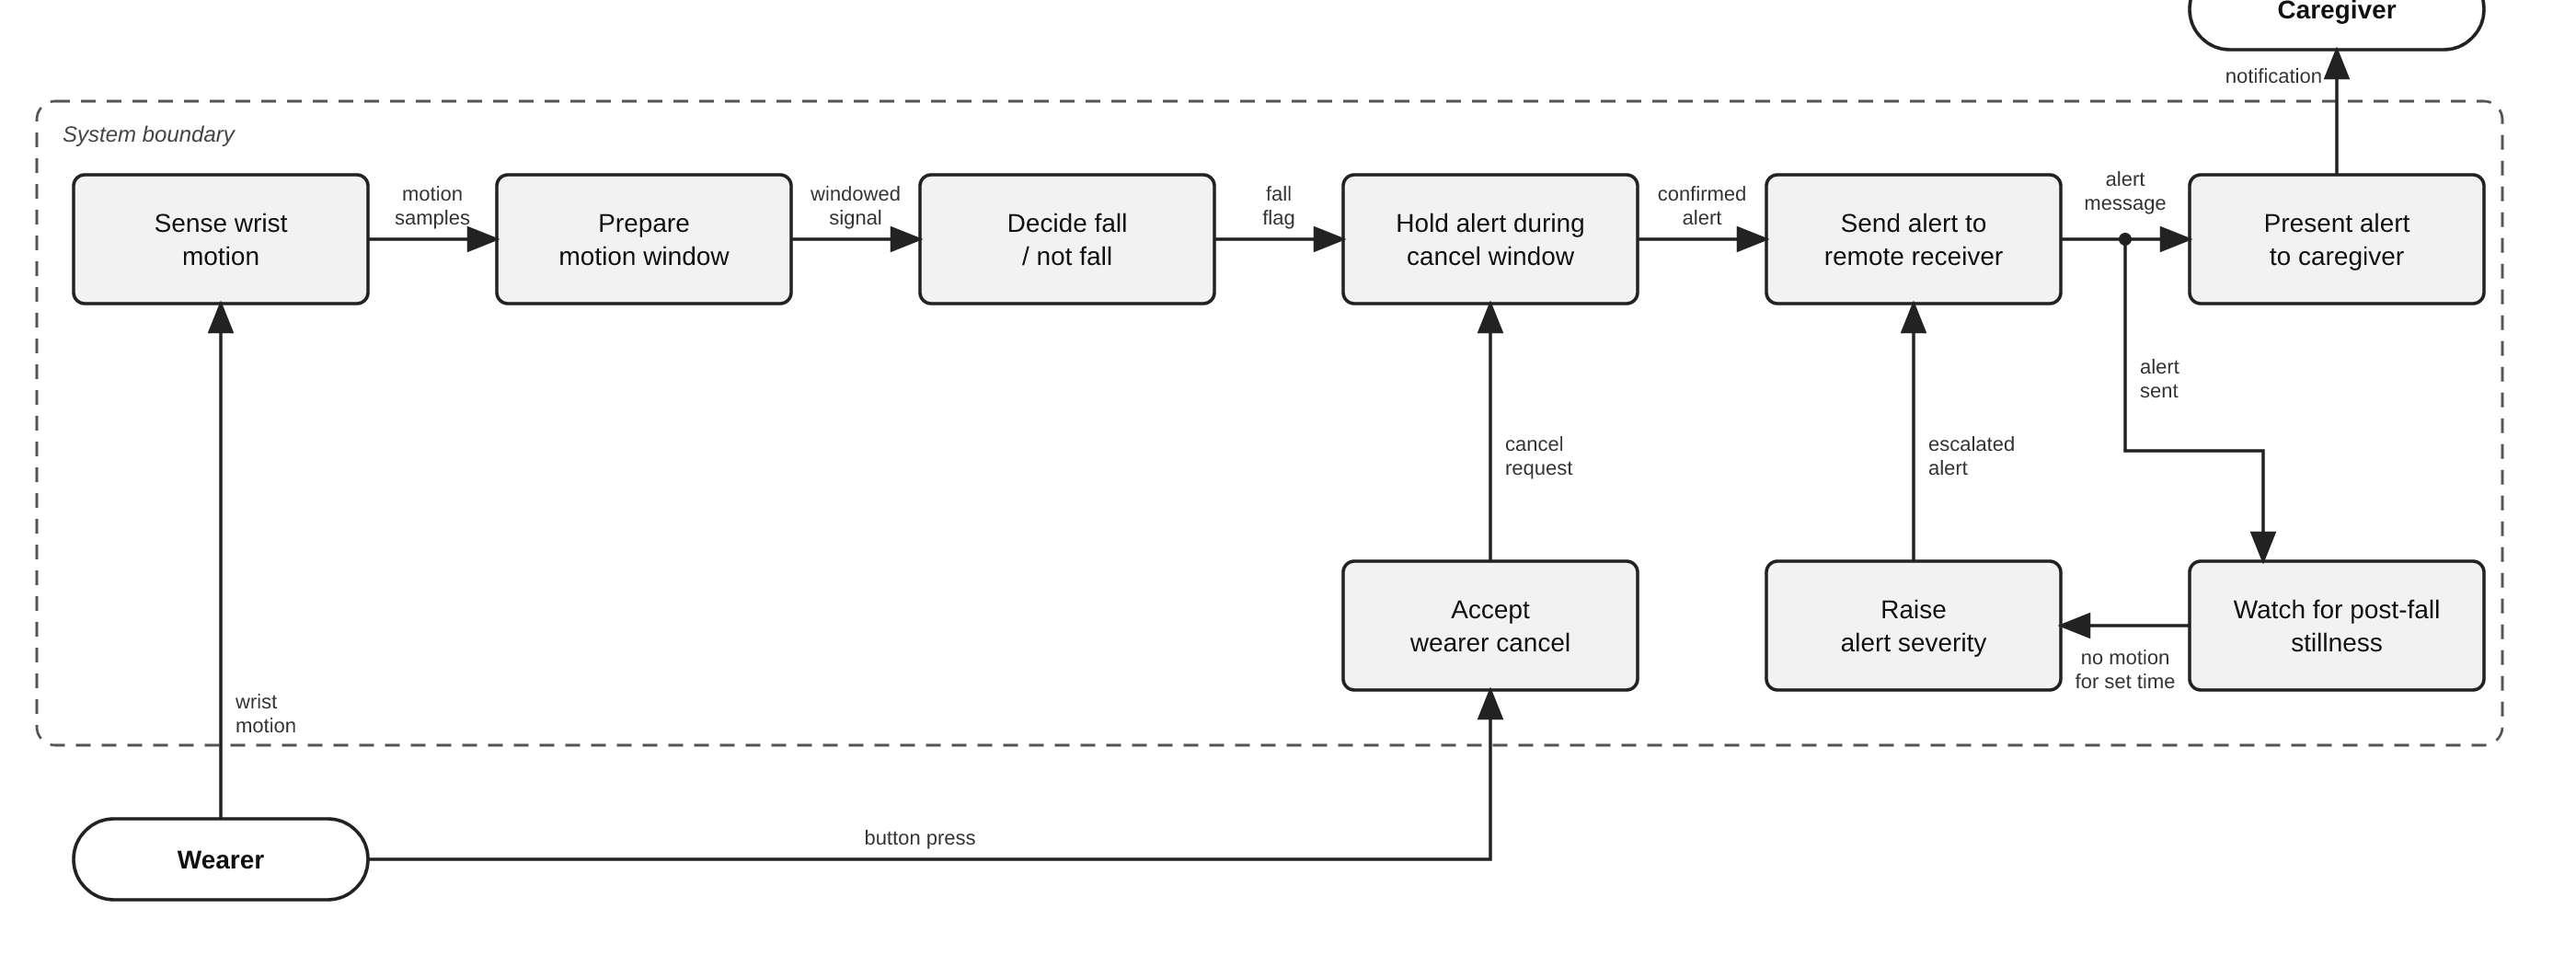
\includegraphics[width=\columnwidth]{figures/generated/concept_a_block_diagram.png}
    \caption{Functional block diagram of concept A (watch only).}
    \label{fig:blocks}
\end{figure}

% ---------------------------------------------------------------
\section{Feasibility Case}
\label{sec:feasibility}

\textbf{Test conditions.} Classifier: random forest on 14 wrist features in a window from 1\,s before to 2\,s after any impact above 2.5\,g, sampled at 238\,Hz, trained on FallAllD (\Lmodel). Model v1 (threshold 0.26) was used in round 1, v2 (0.30) from round 2 on. One wearer (myself), scripted falls and non-fall movements, each trial marked on the watch with the BOOT button and logged to an SD card. Alert path: watch, MQTT over Wi-Fi, broker on a laptop, Raspberry Pi display. The Pi acknowledges each message and the watch resends until it does. Delivery delay runs from detection on the watch to arrival at the Pi and includes the 15\,s cancel window. All logs and scripts can be found in the project repository.

% Source file for Table 3.
% Required in order for the reference in "gate1_report.tex" to work properly.

\begin{table*}[!tb]
\centering
\scriptsize
\renewcommand{\arraystretch}{1.1}
\setlength{\tabcolsep}{4pt}
\caption{Detection trials on the wearer (measured). Each FALL call inside a trial window counts once. Round 3 is not concept A.}
\label{tab:rounds}
\begin{tabularx}{\linewidth}{@{}l l c c Y@{}}
\toprule
Round (entry) & Model & Falls detected & Non-fall false alarms & Non-fall movements \\
\midrule
1 (\Lrone) & v1, wrist & 19 of 20 & 8 of 10 (80\%) & mixed daily movements \\
2 (\Lrtwo) & v2, wrist & 20 of 20 & 11 of 20 (55\%) & mixed daily movements \\
3 (\Lrthree), waist board comparison & fused wrist + waist & 20 of 20 & 11 of 20 (55\%); wrist alone on the same impacts 18 of 20 & sitting down hard, hard arm swings, wrist hitting a table or the body \\
\bottomrule
\end{tabularx}
\end{table*}



% Source file for Table 4.
% Required in order for the reference in "gate1_report.tex" to work properly.

\begin{table*}[!tb]
\centering
\scriptsize
\renewcommand{\arraystretch}{1.15}
\setlength{\tabcolsep}{2.5pt}
\caption{The feasibility case for concept A.}
\label{tab:claims}
\begin{tabularx}{\linewidth}{@{}L{0.04} L{0.075} L{0.25} c L{0.075} Y L{0.1}@{}}
\toprule
ID & Tests & Claim & Class & Source & Evidence & Status \\
\midrule
CL1 & REQ-FD-01 & A detected fall raises an alert with no wearer action. & Measured & \Lall & All trials trigger in the link runs started an alert without input. & Supported \\
CL2 & REQ-FD-03 & The miss rate is at most 5\% on held-out falls. & Measured & \Lrone, \Lrtwo & 0 of 20 missed in round 2 (round 1: 1 of 20). One wearer and 20 falls: no misses observed, but too few trials to confirm the 5\% target. & Supported (limited power) \\
CL3 & REQ-FD-04 & The false-alarm rate is below 10\% on held-out non-falls. & Measured & \Lrone, \Lrtwo & 11 of 20 (55\%) in round 2, 8 of 10 in round 1. False alarms are sharp wrist impacts followed by stillness. & Unsupported \\
CL4 & REQ-FD-02 & Alerts arrive within 25\,s on strong and weak links. & Measured & \Llinkone, \Llinktwo & Strong: 10 of 10, 15.2--15.4\,s. Weak, no resend: 9 of 10, one lost. Weak, with resend: 10 of 10, up to 24.5\,s (one delay unknown, clock not synced). Moderate: 10 of 10, 15.0--15.1\,s. 10 trials per link, not the 20 planned. & Partly supported \\
CL5 & REQ-FD-05 & A button press within 15\,s cancels the alert. & Measured & \Lrtwo, \Lmqtt & 31 presses in round 2, 1.9--7.5\,s after detection, all cancelled; uncancelled alerts were sent at 15\,s. & Supported \\
CL6 & REQ-FD-06 & 60\,s without motion after a fall raises the severity. & Measured & \Lmqtt & Watch dropped and left still: 5 of 5 escalated at 60.0\,s of stillness. Picked up and moved: 5 of 5 did not. Bench trials, not worn. & Supported \\
CL7 & REQ-FD-07 & Prototype hardware costs at most \$200. & Calculated & \Lcost & Watch \$51.64 (purchased in a group with classmates). Waist board receipts not yet added. & Partly supported \\
CL8 & REQ-FD-08 & Firmware builds and flashes on a fresh machine with no edits. & Measured & -- & Not yet tried. To check before Gate 2. & Open \\
CL9 & C4 & The watch runs the classifier in real time. & Measured & \Lall & Ran on every trial since round 1. Raw logs from the post-fall, moderate-link and round 3 sessions (57.6\,min): 238.0\,Hz held, longest gap between samples 7\,ms, with Wi-Fi and SD logging running and, in round 3, Bluetooth. & Supported \\
CL10 & REQ-FD-06, R2 & Rest alone cannot escalate: escalation only follows a fall alert the wearer did not cancel. & Measured & \Lpost & Cancelling ends the post-fall check. Round 3: 31 alarms cancelled (20 falls, 11 false alarms), 0 escalations. After an alert is sent, BOOT (``I'm OK'') stops escalation at any time. & Supported \\
CL11 & REQ-FD-02 & Alerts still arrive after a broker outage. & Measured & \Llinktwo & Broker stopped 10--15\,s: 5 of 5 delivered, 28--40\,s. Suspended about 20\,s: 5 of 5, 35--61\,s. No restarts. All above 25\,s. & Partly supported \\
\bottomrule
\end{tabularx}
\end{table*}


\textbf{What the shortfalls mean.} The detection path works and missed no falls in round 2, but false alarms are five times the limit, so concept A as tested cannot meet REQ-FD-04 (CL3). Most false alarms are sharp wrist impacts followed by stillness, which a wrist sensor cannot tell apart from a fall; this is the weakness concept A was scored down for. Delivery is reliable once messages are acknowledged and resent: every alert arrived, and on links that stayed connected all known delays were within 25\,s (CL4). A broker outage longer than the 10\,s margin pushes delivery past 25\,s (CL11, R4).

\textbf{Waist board comparison (not part of concept A).} To check concept C's assumed coverage advantage, I built a breadboard waist board (ESP32, MPU6050 and BMP280) that sends the watch 14 motion features and a barometric height change over Bluetooth LE after each impact. If it does not answer within 1.2\,s, the watch decides with the wrist alone. In offline testing on FallAllD (calculated, leave-one-subject-out, with at most 5\% of falls missed), false alarms were 7.7\% with the wrist alone and 2.6\% with the waist and barometer added. In round 3 (Table~\ref{tab:rounds}), I wore the waist board and the watch logged, for every impact, the probability from the fused model and from the wrist-only model. Both models therefore scored the same 20 non-fall movements: the fused model raised 11 false alarms and the wrist-only model raised 18. These movements were harsher than round 2's, so the two rounds' rates cannot be compared directly. The board-to-watch delay was 193--476\,ms (median 331\,ms for falls, 347\,ms for non-falls). That exceeds the 200\,ms sub-budget in REQ-FD-02's rationale, although it is under 0.5\,s of the 25\,s total. These results are not claims for concept A; they inform the concept choice for Gate 2 (Sec.~\ref{sec:readiness}).

% ---------------------------------------------------------------
\section{Baselined Requirements}
\label{sec:baseline}

Every requirement is kept as written. None of the shortfalls comes with a reason from the need to change a number, so each is reported against its original line.

% Source file for Table 5.
% Required in order for the reference in "gate1_report.tex" to work properly.

\begin{table*}[!tb]
\centering
\scriptsize
\renewcommand{\arraystretch}{1.15}
\setlength{\tabcolsep}{3pt}
\caption{Baselined requirements. Statements unchanged from the proposal.}
\label{tab:baseline}
\begin{tabularx}{\linewidth}{@{}L{0.075} L{0.27} L{0.07} L{0.11} Y@{}}
\toprule
ID & Statement & Decision & Status & Reason \\
\midrule
REQ-FD-01 & Alert initiated on fall, no wearer action. & Keep & Supported & CL1. \\
REQ-FD-02 & Alert delivered within 25\,s, including over a degraded link; board-to-watch sub-budget 200\,ms. & Keep & Partly supported & Met on connected links (CL4) at 10 trials, not 20. Outages exceed it (CL11). The 200\,ms board-to-watch sub-budget does not apply to concept A; in the waist board comparison it was exceeded, and faster Bluetooth settings (R3's mitigation) will be tried before any revision. \\
REQ-FD-03 & Miss rate $\leq$ 5\%. & Keep & Supported & CL2, limited power. \\
REQ-FD-04 & False-alarm rate $<$ 10\%. & Keep & Unsupported & The need (N3) has not changed, so the limit stays. The design falls short, not the number (CL3). \\
REQ-FD-05 & Cancel by button within 15\,s. & Keep & Supported & CL5. \\
REQ-FD-06 & Escalate after 60\,s without post-fall motion. & Keep & Supported & CL6, CL10. Tested on a dropped watch; a worn wrist lying still is to be checked (R7). \\
REQ-FD-07 & Prototype hardware cost $\leq$ \$200. & Keep & Partly supported & CL7; watch cost calculated but waist board receipts remain outstanding. \\
REQ-FD-08 & Firmware builds and flashes from a clean checkout, no edits. & Keep & Open & CL8, before Gate 2. \\
\bottomrule
\end{tabularx}
\end{table*}


% ---------------------------------------------------------------
\section{Risk Register}
\label{sec:risks}

Each risk is ranked by $P = p \times c$, with $p$ from 1 (rare) to 4 (almost certain) and $c$ from 1 (negligible) to 4 (severe); ties break toward the higher consequence (Table~\ref{tab:risks}, Fig.~\ref{fig:matrix}).

% Source file for Table 6.
% Required in order for the reference in "gate1_report.tex" to work properly.

\begin{table*}[!tb]
\centering
\scriptsize
\renewcommand{\arraystretch}{1.15}
\setlength{\tabcolsep}{3pt}
\caption{Ranked risks and what changed since the proposal.}
\label{tab:risks}
\begin{tabularx}{\linewidth}{@{}l L{0.33} c c c c Y@{}}
\toprule
ID & Risk & $p$ & $c$ & $P$ & Rank & Since the proposal \\
\midrule
R1 & Miss or false-alarm targets not met on new people and sessions. & 4 & 3 & 12 & 1 & Was likely. False alarms now measured at 55\% (CL3). \\
R4 & Broker unavailable for more than 10\,s delays alerts past 25\,s. & 2 & 4 & 8 & 2 & New: outage tests gave 28--61\,s (CL11). \\
R3 & Bluetooth delay exceeds the 200\,ms sub-budget. & 4 & 2 & 8 & 3 & Was unlikely; occurred in the waist board comparison (193--476\,ms). Effect on 25\,s is small. \\
R7 & An unconscious wearer's wrist does not read as still (worn-wrist noise, being moved), so escalation never fires. & 2 & 3 & 6 & 4 & New: stillness tested only on a dropped watch. Escalation is meant for an unconscious wearer to receive help urgently; one who moves on the ground gets the normal alert. \\
R5 & Waist board unavailable (battery, reset, link), so the watch falls back to the wrist and false alarms rise. & 3 & 2 & 6 & 5 & New: one 1.2\,s timeout in testing; the board must be still at power-on. \\
R2 & 60\,s of stillness does not separate incapacitation from rest. & 2 & 2 & 4 & 6 & Was likely. Rest alone cannot escalate: only an uncancelled fall alert starts the check, and the wearer can stop it (CL10). \\
R6 & Watch restarts while reconnecting to Wi-Fi and loses its session. & 1 & 4 & 4 & Closed & New: one watchdog restart on the weak link; fixed by lowering the network task priority, no restarts in three runs since (\Llinktwo). \\
\bottomrule
\end{tabularx}
\end{table*}


\begin{figure}[!t]
\centering
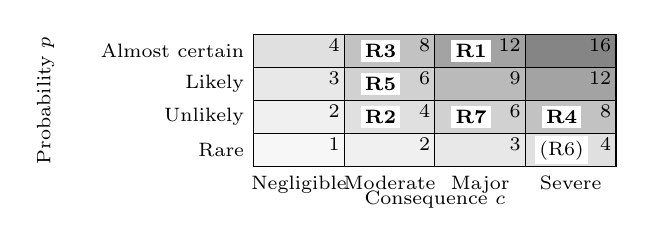
\begin{tikzpicture}[x=1.15cm,y=0.42cm,font=\scriptsize]
  \foreach \p in {1,...,4} {
    \foreach \c in {1,...,4} {
      \pgfmathtruncatemacro{\P}{\p*\c}
      \pgfmathtruncatemacro{\shade}{\P*3}
      \fill[black!\shade] (\c-1,\p-1) rectangle (\c,\p);
      \draw (\c-1,\p-1) rectangle (\c,\p);
      \node[anchor=north east,inner sep=1.5pt] at (\c,\p) {\P};
    }
  }
  \foreach \lab [count=\i] in {Rare,Unlikely,Likely,Almost certain} \node[anchor=east] at (0,\i-0.5) {\lab};
  \foreach \lab [count=\i] in {Negligible,Moderate,Major,Severe} \node[anchor=north] at (\i-0.5,0) {\lab};
  \node[rotate=90] at (-2.3,2) {Probability $p$};
  \node at (2,-1.0) {Consequence $c$};
  \node[font=\scriptsize\bfseries,fill=white,inner sep=1.5pt] at (2.4,3.5) {R1};
  \node[font=\scriptsize\bfseries,fill=white,inner sep=1.5pt] at (1.4,3.5) {R3};
  \node[font=\scriptsize\bfseries,fill=white,inner sep=1.5pt] at (2.4,1.5) {R7};
  \node[font=\scriptsize\bfseries,fill=white,inner sep=1.5pt] at (1.4,1.5) {R2};
  \node[font=\scriptsize\bfseries,fill=white,inner sep=1.5pt] at (1.4,2.5) {R5};
  \node[font=\scriptsize\bfseries,fill=white,inner sep=1.5pt] at (3.4,1.5) {R4};
  \node[font=\scriptsize,fill=white,inner sep=1.5pt] at (3.4,0.5) {(R6)};
\end{tikzpicture}
\caption{Risk matrix. Each cell shows $P = p \times c$; darker cells come first. R6 is closed.}
\label{fig:matrix}
\end{figure}

% Source file for Table 7.
% Required in order for the reference in "gate1_report.tex" to work properly.

\begin{table}[!t]
\centering
\scriptsize
\renewcommand{\arraystretch}{1.15}
\setlength{\tabcolsep}{3pt}
\caption{The two top-ranked risks in full.}
\label{tab:toprisks}
\begin{tabularx}{\linewidth}{@{}L{0.14} Y Y@{}}
\toprule
Field & R1 & R4 \\
\midrule
Statement & Miss or false-alarm targets are not met on new people and sessions. & The broker is unavailable for more than 10\,s, so alerts arrive after 25\,s. \\
Assumption & A model trained on FallAllD subjects carries over to a new wearer and real movements. & The broker on the laptop is running and reachable whenever the watch has an alert. \\
Consequence & Frequent false alarms make the wearer stop wearing it (N3), or falls go undetected (N1). & The caregiver is told late (N4, N7) and REQ-FD-02 is missed. \\
Probability & Almost certain: 11 of 20 and 8 of 10 false alarms on held-out sessions. Misses so far 0 of 20 in round 2. & Unlikely: no unplanned outage in any session; forced outages of 10--20\,s gave 28--61\,s, with every alert delivered (CL11). \\
Evidence Required & Under 10\% false alarms on 20 held-out non-fall trials with each movement labelled, including a second person. & Delivery times over long sessions with the broker on the machine it would run on in use. \\
Mitigation & Carry the fused wrist and waist model forward (waist board comparison, Sec.~\ref{sec:feasibility}); add confusable movements to training; label every trial. & Run the broker on an always-on device such as the Pi; keep resend until acknowledged. \\
\bottomrule
\end{tabularx}
\end{table}


% ---------------------------------------------------------------
\section{Gate 1 Readiness}
\label{sec:readiness}

The watch-only concept detects falls and delivers alerts as designed. It raised an alert without input on all link-test triggers (CL1), missed none of 20 worn falls in round 2 (CL2), sent every alert within 25\,s on links that stayed connected (CL4), let the wearer cancel (CL5), escalated after 60\,s of stillness (CL6), and kept its 238\,Hz sampling while doing all of this (CL9). It does not meet the false-alarm requirement: 55\% against a limit of 10\% (CL3), which makes R1 the top risk. The waist board comparison shows that a second sensor removes some of these false alarms (18 to 11 of 20 on the same movements), but not enough, and that its Bluetooth delay exceeds the 200\,ms sub-budget while hardly affecting the 25\,s total. Still open: whether an unconscious wearer's worn wrist reads as still (R7), waist board costs (CL7), and the clean-checkout build (CL8).

I expect \textbf{proceed with conditions}. The evidence supports the alert path and the detection of falls, and it locates the false-alarm problem precisely enough to work on. I would accept these conditions for Gate 2: (1) bring the false-alarm rate under 10\% on 20 labelled held-out non-fall trials, or re-scope, with the coverage criterion re-scored using the measured fusion result; (2) run worn trials lying fully still after a fall, standing in for unconsciousness/incapacitation, to settle R7; (3) repeat the delivery tests at 20 trials per link condition and try shorter Bluetooth connection intervals against the 200\,ms sub-budget; (4) add the waist board receipts and complete a build on a second machine.

\textbf{AI-assisted steps.} An AI assistant wrote most of the testing firmware and scripts, scored the logs and assisted in the creation of this report; I checked every figure against my logs and logbook.

\end{document}
